\documentclass[11pt]{article}

% Change "review" to "final" to generate the final (sometimes called camera-ready) version.
% Change to "preprint" to generate a non-anonymous version with page numbers.
\usepackage[review]{acl}
%\usepackage[preprint]{acl}
% Standard package includes
\usepackage{times}
\usepackage{latexsym}
\usepackage{makecell}

\usepackage{tikz}
\usetikzlibrary{arrows.meta,positioning}

\usepackage{pgfplots}
\pgfplotsset{compat=1.18}
\usepackage{booktabs}
\usepackage{multirow}
\usepackage{xcolor}
\usepackage{colortbl}
% 定义一些强调色，用于Highlight SOTA
\newcommand{\best}[1]{\textbf{\textcolor{blue!70!black}{#1}}} % SOTA
\newcommand{\better}[1]{\underline{#1}} % 超过金牌线
\newcommand{\RankOne}[1]{\textbf{\textcolor{yellow!50!orange}{#1}}}
\newcommand{\RankTwo}[1]{\textbf{\textcolor{cyan}{#1}}}
\newcommand{\RankThree}[1]{\textbf{\textcolor{lime!80!black}{#1}}}
\newcommand{\strong}[1]{\textbf{\textcolor{red!70!black}{#1}}} % SOTA

\newcommand{\golden}[1]{\textbf{\textcolor{yellow!90!black}{#1}}} % SOTA
\newcommand{\ContamV}[1]{\multicolumn{1}{!{\color{red!75!black}\vrule width 1.2pt}r}{#1}}


% Preamble (optional)
\usepackage[most]{tcolorbox}
\usepackage{booktabs}
\usepackage{enumitem}
\newcommand{\pts}[1]{\qquad{\small(#1 pts)}}
% Preamble (add if not already in your ACL file)
\usepackage{booktabs}
\usepackage{pifont}
\newcommand{\cmark}{\ding{51}}
\newcommand{\xmark}{\ding{55}}

% in preamble
\usepackage{booktabs}
\usepackage{tabularx}
\usepackage{array}

% nicer TabularX "X" column (left-aligned, allows \newline)
\newcolumntype{Y}{>{\raggedright\arraybackslash}X}

% --- Consistent two-line card header ---
\newcommand{\CardHeader}[2]{%
\begin{tabular}{@{}l@{}}
{\Large\bfseries #1}\\[-0.15em]
{\normalsize\itshape #2}
\end{tabular}
}


% For proper rendering and hyphenation of words containing Latin characters (including in bib files)
\usepackage[T1]{fontenc}
% For Vietnamese characters
% \usepackage[T5]{fontenc}
% See https://www.latex-project.org/help/documentation/encguide.pdf for other character sets

% This assumes your files are encoded as UTF8
\usepackage[utf8]{inputenc}

% This is not strictly necessary, and may be commented out,
% but it will improve the layout of the manuscript,
% and will typically save some space.
\usepackage{microtype}

% This is also not strictly necessary, and may be commented out.
% However, it will improve the aesthetics of text in
% the typewriter font.
\usepackage{inconsolata}

%Including images in your LaTeX document requires adding
%additional package(s)
\usepackage{graphicx}
% Resolve figures both when the project root or this latex/ directory is the build root.
\graphicspath{{./}{latex/}}
\usepackage{caption} % for \captionof inside tcolorbox (no floats)

% If the title and author information does not fit in the area allocated, uncomment the following
%
%\setlength\titlebox{<dim>}
%
% and set <dim> to something 5cm or larger.

\newcommand{\medal}[1]{\raisebox{-0.25\height}{\includegraphics[height=1.15em]{#1}}}

\newcommand{\WinnerMedal}{\medal{medal/trophy.png}}
\newcommand{\GoldMedal}{\medal{medal/gold.png}}
\newcommand{\SilverMedal}{\medal{medal/silver.png}}
\newcommand{\BronzeMedal}{\medal{medal/bronze.png}}
\newcommand{\ClownMedal}{\medal{medal/clown.png}}


% 在数字后面加 medal
\newcommand{\Winner}[1]{\WinnerMedal\,#1}
\newcommand{\Gold}[1]{\GoldMedal\,#1}
\newcommand{\Silver}[1]{\SilverMedal\,#1}
\newcommand{\Bronze}[1]{\BronzeMedal\,#1}
\newcommand{\Clown}[1]{\ClownMedal\,#1}


\title{ScienceArena: Benchmarking LLMs on Latest Scientific Olympiad Competitions}

% Author information can be set in various styles:
% For several authors from the same institution:
% \author{Author 1 \and ... \and Author n \\
%         Address line \\ ... \\ Address line}
% if the names do not fit well on one line use
%         Author 1 \\ {\bf Author 2} \\ ... \\ {\bf Author n} \\
% For authors from different institutions:
% \author{Author 1 \\ Address line \\  ... \\ Address line
%         \And  ... \And
%         Author n \\ Address line \\ ... \\ Address line}
% To start a separate ``row'' of authors use \AND, as in
% \author{Author 1 \\ Address line \\  ... \\ Address line
%         \AND
%         Author 2 \\ Address line \\ ... \\ Address line \And
%         Author 3 \\ Address line \\ ... \\ Address line}

\author{xxx \\
  \texttt{email@domain} \\\And
  xxx \\
  \texttt{email@domain} \\}

%\author{
%  \textbf{First Author\textsuperscript{1}},
%  \textbf{Second Author\textsuperscript{1,2}},
%  \textbf{Third T. Author\textsuperscript{1}},
%  \textbf{Fourth Author\textsuperscript{1}},
%\\
%  \textbf{Fifth Author\textsuperscript{1,2}},
%  \textbf{Sixth Author\textsuperscript{1}},
%  \textbf{Seventh Author\textsuperscript{1}},
%  \textbf{Eighth Author \textsuperscript{1,2,3,4}},
%\\
%  \textbf{Ninth Author\textsuperscript{1}},
%  \textbf{Tenth Author\textsuperscript{1}},
%  \textbf{Eleventh E. Author\textsuperscript{1,2,3,4,5}},
%  \textbf{Twelfth Author\textsuperscript{1}},
%\\
%  \textbf{Thirteenth Author\textsuperscript{3}},
%  \textbf{Fourteenth F. Author\textsuperscript{2,4}},
%  \textbf{Fifteenth Author\textsuperscript{1}},
%  \textbf{Sixteenth Author\textsuperscript{1}},
%\\
%  \textbf{Seventeenth S. Author\textsuperscript{4,5}},
%  \textbf{Eighteenth Author\textsuperscript{3,4}},
%  \textbf{Nineteenth N. Author\textsuperscript{2,5}},
%  \textbf{Twentieth Author\textsuperscript{1}}
%\\
%\\
%  \textsuperscript{1}Affiliation 1,
%  \textsuperscript{2}Affiliation 2,
%  \textsuperscript{3}Affiliation 3,
%  \textsuperscript{4}Affiliation 4,
%  \textsuperscript{5}Affiliation 5
%\\
%  \small{
%    \textbf{Correspondence:} \href{mailto:email@domain}{email@domain}
%  }
%}

\begin{document}
\maketitle
\begin{abstract}
Benchmark saturation and public-data exposure increasingly obscure scientific reasoning in frontier LLMs. We introduce \textsc{ScienceArena}, an olympiad-style benchmark built from public physics, chemistry, and biology competitions with multi-step answers and process credit. A provenance-audited pipeline converts available exams, figures, solutions, and marking material into structured turns while retaining source and rubric provenance. We calibrate automated grading against medalist scores on archived IPhO and IChO 2025 answers, then separately evaluate a newly reconstructed 2026 panel containing IPhO, IChO, NBPhO, and USAPhO. Route modality is frozen before scoring: eight vision-verified routes receive native question text and byte-preserving encodings of official question-page PNGs, whereas six text-only routes receive an answer-blind question staticization and no image blocks. A strict image-aware judge scores visible answers against official marking rules where available and solution-derived criteria otherwise; every request, validation decision, and terminal score is retained for replay. The four-contest panel contains 2,142 terminal model--turn scores and no missing model--contest cells. These are measurements on public exams: route-specific availability dates and training exposure are not established, so we do not present the panel as an uncontaminated holdout. We provide an interactive demo at \url{https://science-arena-review.onrender.com/}.
\end{abstract}


\section{Introduction}
Scientific reasoning has become a central target for frontier LLMs, yet evaluation is at an impasse.
Popular benchmarks are increasingly saturated and vulnerable to contamination \citep{hendrycks2021mmlu,li2023contamination,rein2023gpqa,white2024livebench,phan2025hle}.
Recent live or frontier benchmarks respond by using time-sensitive sources, contest problems, or newly authored expert questions \citep{jain2024livecodebench,glazer2024frontiermath,balunovic2025matharena}, but scientific reasoning remains difficult to measure when answers are long, visual, and partially correct.
At the same time, many science evaluations remain confined to short-answer or multiple-choice formats, which cannot fully test the abilities needed in real scientific problem solving: long derivations, diagram and structure interpretation, multi-step consistency, and partial credit under explicit rubrics \citep{wang2023scibench,lu2023mathvista,yue2023mmmu,he2024olympiadbench,lu2022scienceqa,laurent2024labbench,mirza2025chembench}.


Science olympiad competitions are a natural high-resolution testbed.
They are written by domain experts and released publicly during or after the contest, often with answers, detailed solutions, or scoring schemes whose provenance varies by competition.
They also provide interpretable human reference points, including gold-medal thresholds and winner scores.
However, turning olympiad exams into a reliable LLM benchmark is not automatic.
The source materials are PDFs with formulas, figures, tables, and chemical structures; more importantly, faithful scoring requires stepwise rubrics and expert judgment rather than simple exact matching.


We present \textsc{ScienceArena}, an olympiad-style benchmark and evaluation protocol for scientific reasoning.
The benchmark index covers 15 contest-year datasets released in 2023--2026: an eleven-dataset legacy suite and a separately reconstructed four-contest 2026 panel. It includes international exams such as IPhO, IChO, and IBO as well as national-level exams such as USAPhO and USNCO.
We standardize the data construction pipeline: public materials are collected, converted into structured JSON with OCR and multimodal parsing, and checked for source, field, figure, and rubric provenance. Medalist grading is limited to the archived IPhO/IChO calibration described below.
Rubric provenance is retained explicitly: we use official marking rules where they are released and label criteria derived from supplied worked solutions otherwise, retaining each solution's provenance status.
This preserves the original exam structure while making the problems readable to text-based and multimodal LLM APIs.



\begin{table*}[t]
\centering
\scriptsize
\setlength{\tabcolsep}{5pt}
\renewcommand{\arraystretch}{0.95}
\begin{tabularx}{\textwidth}{p{0.19\textwidth} p{0.23\textwidth} Y}
\toprule
\textbf{Benchmark} & \textbf{Main signal} & \textbf{ScienceArena distinction} \\
\midrule
Chatbot Arena; Arena-Hard
& Human or judge preference
& Tests verifiable scientific correctness rather than broad helpfulness. \\
\addlinespace[0.12em]
\makecell[l]{OlympicArena/\\OlympiadBench}
& Cross-discipline hard reasoning
& Keeps recent science exams, release metadata, provenance-labelled criteria, and archived medalist calibration. \\
\addlinespace[0.12em]
MathArena
& Fresh math answers/proofs
& Adds physics, chemistry, biology, diagrams, structures, and science process credit. \\
\addlinespace[0.12em]
\makecell[l]{HiPhO/PhyArena/\\PhysicsArena}
& Physics olympiad or skill axes
& Adds a route-aware public physics/chemistry panel and a legacy objective biology track. \\
\addlinespace[0.12em]
SUPERChem; BABE
& Domain research or expert tasks
& Uses public competition material with provenance-labelled criteria and selected human references. \\
\addlinespace[0.12em]
SciArena
& Researcher preference
& Scores against answers and criteria labelled official where released and solution-derived otherwise. \\
\midrule
\textsc{ScienceArena}
& Release-aware olympiad scoring
& Combines provenance-labelled credit criteria, calibrated judges, and archived expert diagnostics. \\
\bottomrule
\end{tabularx}
\vspace{-0.1cm}
\caption{Positioning of \textsc{ScienceArena} among representative Arena-style and domain-specific evaluations. The comparison highlights release-aware science olympiad evaluation with official criteria where released, solution-derived criteria otherwise, and archived medalist diagnostics.}
\label{tab:arena-positioning}
\vspace{-0.4cm}
\end{table*}




Table~\ref{tab:arena-positioning} positions \textsc{ScienceArena} relative to recent Arena-style and domain-specific evaluations.
General-purpose arenas such as Chatbot Arena and Arena-Hard emphasize human or judge-model preferences over open-ended assistant behavior \citep{chiang2024chatbotarena,li2024arenahard}.
Olympiad and competition benchmarks provide harder reasoning tasks, including OlympicArena, OlympiadBench, and MathArena \citep{huang2024olympicarena,he2024olympiadbench,balunovic2025matharena}.
The closest physics-only line is HiPhO/PhyArena, which uses latest physics olympiad exams and official medal thresholds \citep{yu2025hipho}; other domain benchmarks decompose physics, chemistry, biology, or scientific literature reasoning with different task sources and scoring signals \citep{dai2025physicsarena,zhao2025superchem,zhou2026babe,zhao2025sciarena}.
Our focus is complementary: recent public olympiad exams across physics, chemistry, and biology, provenance-labelled process-credit criteria, selected human reference points, source/rubric auditing, and expert-calibrated automated grading.






A second challenge is evaluation cost.
Human olympiad experts provide the most reliable ground truth, but repeatedly asking them to grade every new model is impractical.
We therefore develop an expert-calibrated LLM-as-judge system.
Using human medalist scores on IPhO 2025 and IChO 2025 as ground truth, we calibrate the full judge system, including rubric packaging, structured scoring, score validation, and aggregation, on archived answers from five models.
Across the four judge--exam combinations, candidate-total mean absolute error is 0.30--0.74 points and the maximum absolute error is 1.00 point. This narrow replay supports practical automated scoring for the stated configuration while retaining an explicit human validity boundary; it is not a cross-family validation.




Finally, we examine how LLMs should solve long olympiad problems.
One-shot prompting asks for an entire multi-part solution at once, while interleaved prompting presents subparts sequentially and preserves prior context.
We do not claim interleaving as a new method; rather, we test this natural prompting choice and find that it generally improves performance and better resembles how users interact with LLMs on difficult problems.
We therefore use interleaved prompting for the main evaluation.
Across fourteen recent LLM routes, the strongest systems obtain high rubric scores on several public exams; we use medal-equivalent language only when a same-year official threshold and matching scale are available.
The gains are uneven across the public four-contest panel, while archived comments highlight visual grounding, long-horizon physical control, molecular structures, stereochemistry, and rubric-sensitive drawings as recurring risks.
Beyond aggregate scores, we study the written comments produced by olympiad medalist graders.
These notes are unusually diagnostic: they distinguish fluent but physically misgrounded derivations from correct problem models, separate chemically plausible prose from exact structure commitments, and expose when partial credit depends on an explicit intermediate rather than a vague explanation.
We use these comments to build the subfield and ability-boundary analysis in Section~\ref{sec:expert-insights} and Appendix~\ref{app:expert_notes}.

\begin{figure*}[htbp]
\centering
\setlength{\abovecaptionskip}{0.1cm}
\resizebox{0.97\textwidth}{!}{%
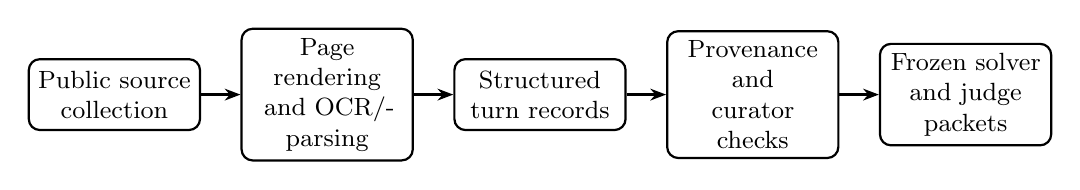
\begin{tikzpicture}[
  node distance=5mm,
  every node/.style={draw,rounded corners,align=center,font=\small,minimum height=9mm,text width=0.16\textwidth},
  every path/.style={-{Stealth[length=2mm]},thick}
]
\node (a) {Public source\\collection};
\node[right=of a] (b) {Page rendering\\and OCR/parsing};
\node[right=of b] (c) {Structured\\turn records};
\node[right=of c] (d) {Provenance and\\curator checks};
\node[right=of d] (e) {Frozen solver\\and judge packets};
\draw (a) -- (b); \draw (b) -- (c); \draw (c) -- (d); \draw (d) -- (e);
\end{tikzpicture}
}
\caption{\textsc{ScienceArena} benchmark construction pipeline. Medalist grading is a separate archived calibration, not a claim about every construction stage.}
\label{fig:benchmark-pipeline}
\vspace{-0.4cm}
\end{figure*}

\paragraph{Contributions.}
We make four contributions:
\begin{itemize}[leftmargin=0.5em,itemsep=0.1em]
    \item We document an eleven-dataset legacy index and release a provenance-audited four-contest panel with questions, figures, answer material, and provenance-labelled scoring criteria.
    \item We define a reusable pipeline for converting official olympiad PDFs into structured LLM-readable benchmark items.
    \item We develop an expert-calibrated LLM-as-judge system that closely matches olympiad-medalist grading on IPhO \& IChO calibration experiments.
    \item We compare one-shot and interleaved prompting, evaluate fourteen recent API routes on a four-contest 2026 panel with complete terminal accounting, and release a provenance-addressed archive of 525 expert-scored rows, including 410 verbatim comments.
\end{itemize}








\section{The ScienceArena Framework}\label{sec:2}
\textsc{ScienceArena} is designed around two constraints that are often absent from standard LLM benchmarks.
First, the source tasks must be recent, public, scientifically meaningful, and accompanied by explicit temporal-risk metadata.
Second, grading must respect olympiad rubrics: a wrong final value may still receive credit for a correct setup, while a correct-looking answer may receive little credit if the derivation or diagram is unsupported.
This section describes the benchmark construction pipeline, the calibrated judge system, and the solving protocols used for the experiments.


\subsection{Benchmark Construction}
\textsc{ScienceArena} currently contains an eleven-dataset legacy archive across physics, chemistry, and biology and a separately frozen four-contest 2026 physics/chemistry panel (Table~\ref{tab:science_arena_sources}).
The contest year is part of the dataset identity: the legacy NBPhO and USAPhO rows are 2025, whereas the current route-aware panel uses their 2026 editions. International competitions can provide human reference thresholds; national-level competitions expand topic diversity and reduce dependence on one exam style.
For every benchmark, we record an evidenced public release date or explicit unknown status and preserve the original hierarchy: each multi-part problem becomes linked turns with text, figure context, answer material, criteria, and maximum score.
This keeps partial-credit structure intact while supporting uniform automated evaluation.


\begin{table}[t]
\centering
\scriptsize
\setlength{\tabcolsep}{3pt}
\renewcommand{\arraystretch}{0.98}
\resizebox{\columnwidth}{!}{
\begin{tabular}{l l l c r}
\toprule
\textbf{Benchmark} & \textbf{Subject} & \textbf{Level} & \textbf{Rel.} & \textbf{Scale} \\
\midrule
IPhO 2025 & Physics & International & 25-07 & 30 \\
IChO 2025 & Chemistry & International & 25-07 & 60 \\
IBO 2023 & Biology & International & 23-07 & 453 \\
APhO 2025 & Physics & Continental & 25-05 & 30 \\
EuPhO 2025 & Physics & Continental & 25-06 & 30 \\
NBPhO 2025 & Physics & National & 25-04 & 72 \\
USAPhO 2025 & Physics & National & 25-04 & 150 \\
CPhO 2025 & Physics & National & 25-10 & 320 \\
INChO 2026 & Chemistry & National & 26-01 & 106 \\
USNCO 2025 & Chemistry & National & 25-06 & 100 \\
CChO 2025 & Chemistry & National & 25-10 & 100 \\
\midrule
IPhO 2026 & Physics & International & 26-? & 30 \\
IChO 2026 & Chemistry & International & 26-? & 60 \\
NBPhO 2026 & Physics & National & 26-04 & 72 \\
USAPhO 2026 & Physics & National & 26-05 & 150 \\
\bottomrule
\end{tabular}
}
\vspace{-0.2cm}
\caption{\textsc{ScienceArena} contest-year datasets. The first block is the legacy text-staticized archive and the second is the frozen 2026 route-aware panel. Release dates use YY-MM; ``?'' means that the official page does not establish an exact release month/day. ``Scale'' is the reported full score; rubric provenance and source caveats are retained per item.}
\label{tab:science_arena_sources}
\vspace{-0.5cm}
\end{table}

\paragraph{Digitization pipeline.}
Olympiad materials are PDFs with equations, plots, molecule drawings, apparatus diagrams, answer images, and marking schemes, so we convert them through a five-stage pipeline.
A curator first collects official public problems, figures, answer keys, solutions, and marking schemes; pages are then rendered and parsed with OCR/multimodal models.
The parsed content is normalized into fields such as \texttt{question\_text}, \texttt{official\_answer}, \texttt{official\_detailed\_solution}, \texttt{official\_rubric}, \texttt{max\_score}, \texttt{release\_date}, and source provenance.
Curator and provenance checks cover completeness, figure alignment, answer fidelity, and point totals; the archived IPhO/IChO medalist calibration is summarized in Table~\ref{tab:human-graders}.
The final export is a unified interleaved dataset with one row per subproblem turn.
Figure~\ref{fig:benchmark-pipeline} summarizes the intended five-stage construction schematic.

We call a question \emph{text-staticized} when its native question text is augmented with a frozen, audited description of question-side visual evidence.
Staticization is not the original image.
For the fresh 2026 evaluation, the question-only staticizer can access official question pages but cannot access answers, solutions, rubrics, or solution images; those fields enter only after solver generation, at grading time.
The legacy staticizer could access answers, solutions, rubrics, and solution images; it therefore violated this answer-blind boundary, even though downstream solver messages contained only staticized text and no image blocks. We do not use those legacy cells as current results.

The audit trail is important because the three sciences stress different failure modes.
Physics often requires plot reading and symbolic carry-over; chemistry depends on reaction schemes, stereochemistry, spectra, and crystal structures; biology is more often objective-keyed but can involve long passages and diagrams.
Preserving sources, parsed text, image-derived descriptions, and audit notes makes these differences inspectable rather than hiding them behind one score.



\begin{table}[ht]
\vspace{-0.2cm}
\centering
\scriptsize
\setlength{\tabcolsep}{4pt}
\renewcommand{\arraystretch}{1.15}
\begin{tabularx}{\columnwidth}{l X X}
\toprule
\textbf{Track} & \textbf{Archived calibration} & \textbf{Scope} \\
\midrule
Physics & Olympiad-medalist grading & IPhO 2025; five candidates \\
\midrule
Chemistry & Olympiad-medalist grading & IChO 2025; five candidates \\
\bottomrule
\end{tabularx}
\caption{Human experts represented in the archived IPhO/IChO ground-truth calibration. The current replay contains five saved candidate solutions per exam; it does not claim broader biology or cross-contest human calibration.}
\label{tab:human-graders}
\vspace{-0.3cm}
\end{table}



\subsection{Expert-Calibrated LLM-as-Judge System}
\label{sec:judge-system}
Human olympiad experts are the strongest graders for open-ended science problems, but they cannot regrade every model update.
We therefore use medalist grading as a calibration anchor and build a reusable LLM-as-judge system for large-scale evaluation.
Table~\ref{tab:human-graders} summarizes the experts recruited by our team for this human ground-truth calibration.







The judge is a pipeline, not a single prompt.
For each non-objective turn, the current production judge receives the question, reference answer, worked solution, provenance-labelled rubric, maximum score, and the candidate's visible response.
It is a fixed vision-verified route: official question-page PNGs are attached first, followed by available official solution or marking-page PNGs; generated image descriptions never replace these judge images.
The judge returns a single JSON object with \texttt{score}, \texttt{max\_score}, frozen criterion identifiers and allocations, exact candidate-evidence quotes, deductions, and an uncertainty flag.
Post-processing uses decimal arithmetic and strict schema, range, criterion, and evidence validation.
Invalid output is rejected and retried for at most seven total wire attempts; no score is clamped and no missing score is synthesized.
For an exhausted case, a versioned, evidence-field-scoped parser may replay only the already stored raw wire responses. It applies frozen transformations in ordered phases, re-runs the complete validator, and accepts the first fully valid attempt in ascending ordinal within the first successful phase; it cannot call the judge again, alter candidate text or criterion allocations, or compose fields across attempts. If no stored response passes, the case remains missing.
Only an exact solver non-answer sentinel is assigned deterministic zero.
Each accepted score therefore remains traceable to a turn packet, criterion, and literal candidate evidence; objective-key items such as IBO are scored deterministically.




\begin{figure}[tbp]
\centering
\setlength{\abovecaptionskip}{0.1cm}

\includegraphics[width=\linewidth]{new-fig/judge_calibration_caption.pdf}
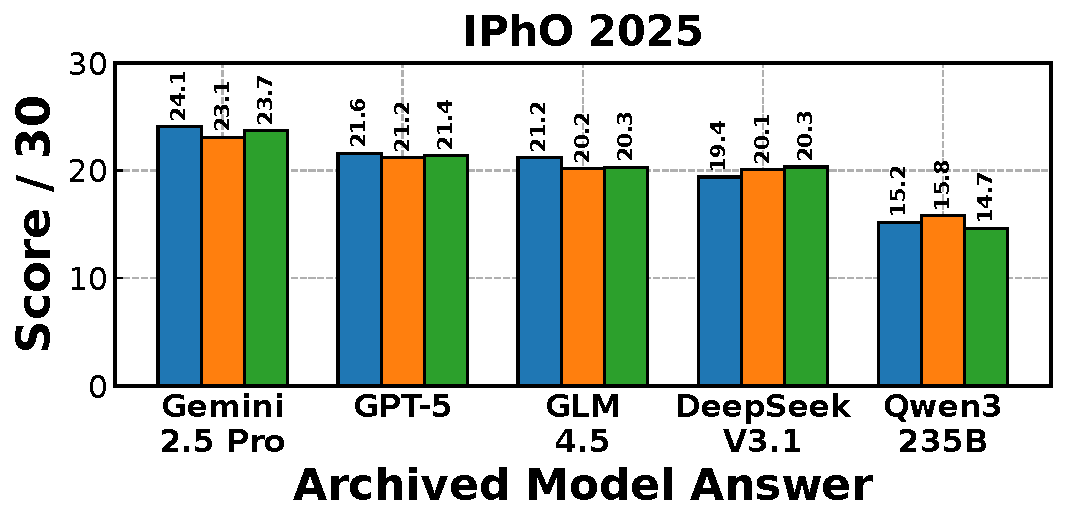
\includegraphics[width=0.93\linewidth]{new-fig/judge_calibration_ipho.pdf}
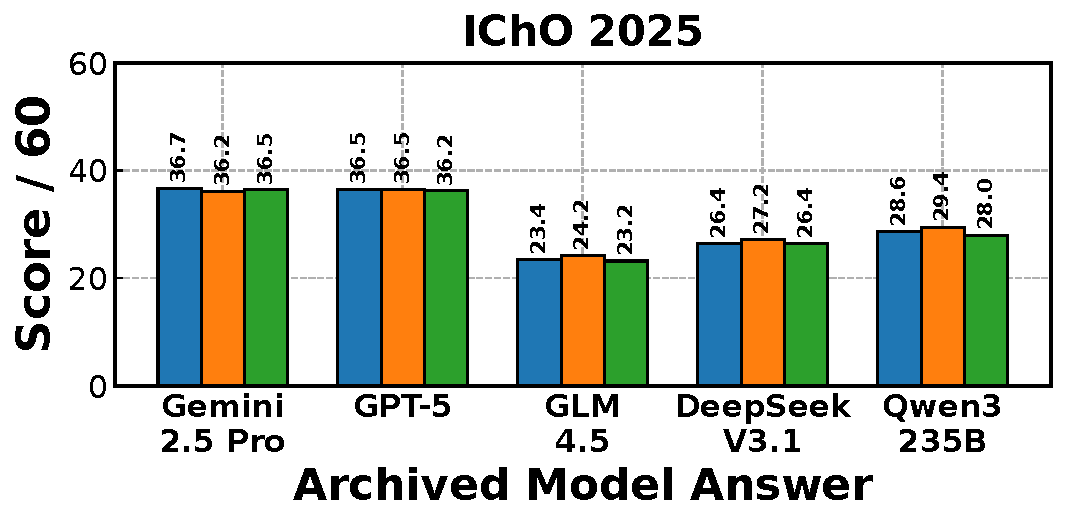
\includegraphics[width=0.93\linewidth]{new-fig/judge_calibration_icho.pdf}
\caption{Calibration of the LLM-as-judge system against human expert ground truth. Blue bars are medalist-assigned candidate totals; the other two bars are scores from the two archived judge replays.}
\label{fig:judge-calibration}
\vspace{-0.3cm}
\end{figure}


We calibrate the system on archived, non-regenerated answers from five models for IPhO 2025 and IChO 2025.
The local replay contains 1,050 judgments over 525 expert-scored rows. Candidate-total MAE is 0.60/0.74 points on IPhO and 0.30/0.56 on IChO for Gemini 3.5 Flash/Gemini 3.1 Pro, with a maximum absolute total error of 1.00 point across the four configurations (Figure~\ref{fig:judge-calibration}). At item level, normalized score MAE ranges from 0.075 to 0.138 and expert--judge Pearson correlation from 0.829 to 0.909.
This result calibrates the historical judge configurations on those saved answers; it does not establish identical error for newer contests, a different route, or the stricter current validator.
The system reached this agreement only after explicitly packaging expert rationales and requiring structured criterion scores. It is a scalable proxy for medalist grading only when the relevant marking material is available, correctly digitized, and covered by the stated calibration boundary.
It shifts the expensive human work from repeatedly grading every model to validating benchmark items and calibrating the judge.







\subsection{Solving Protocols}
\label{sec:solving-protocols}
Physics and chemistry exams often contain dependent subparts, so we compare two prompting protocols.
In \textbf{one-shot} solving, the model receives the full problem and writes one complete solution.
In \textbf{interleaved} solving, it answers one subpart at a time while previous turns remain in context.
Interleaving is not a new algorithm; it is a natural chat interaction pattern whose effect we test directly.
At turn $t$, context contains the earlier questions and the model's own prior visible answers; no reference answer or correction is injected.
Vision-verified routes also retain de-duplicated official question-page images, whereas text-staticized routes always receive zero image blocks.
A turn that still lacks a concrete answer after seven total wire attempts is recorded with a fixed failure sentinel, receives zero, and does not prevent later turns from being attempted.


\begin{figure}[t]
\setlength{\abovecaptionskip}{0.1cm}
\centering
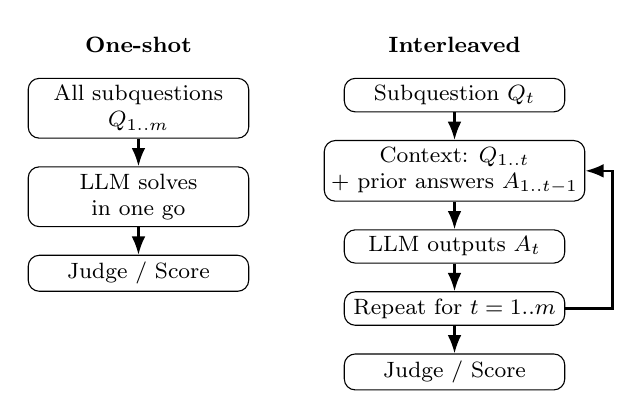
\begin{tikzpicture}[
  font=\footnotesize,
  >={Latex[length=2mm]},
  node distance=3.5mm and 10mm,
  box/.style={draw, rounded corners, align=center, inner sep=2.5pt, minimum width=28mm},
  line/.style={-Latex, thick}
]

% --- One-shot (left) ---
\node[box] (A0) {All subquestions\\$Q_{1..m}$};
\node[box, below=of A0] (A1) {LLM solves\\in one go};
\node[box, below=of A1] (A2) {Judge / Score};
\draw[line] (A0) -- (A1);
\draw[line] (A1) -- (A2);
\node[above=2mm of A0, font=\footnotesize\bfseries] {One-shot};

% --- Iterative (right) ---
\node[box, right=12mm of A0.north east, anchor=north west] (B0) {Subquestion $Q_t$};
\node[box, below=of B0] (B1) {Context: $Q_{1..t}$\\+ prior answers $A_{1..t-1}$};
\node[box, below=of B1] (B2) {LLM outputs $A_t$};
\draw[line] (B0) -- (B1);
\draw[line] (B1) -- (B2);

% loop + final scoring (compact)
\node[box, below=of B2] (B3) {Repeat for $t=1..m$};
\node[box, below=of B3] (B4) {Judge / Score};
\draw[line] (B2) -- (B3);
\draw[line] (B3) -- (B4);
\draw[line] (B3.east) -- ++(6mm,0) coordinate (loop)
            -- (loop |- B1.east) -- (B1.east);


\node[above=2mm of B0, font=\footnotesize\bfseries] {Interleaved};

\end{tikzpicture}
\caption{One-shot vs. interleaved solving schematic.}
\label{fig:one-shot-vs-iterative}
\vspace{-0.3cm}
\end{figure}

Figure~\ref{fig:one-shot-vs-iterative} illustrates the two protocols, and Table~\ref{tab:oneshot-interleaved-ablation} reports the ablation.
Interleaving has the higher point estimate in 15 of 16 archived model--exam comparisons, including all tested IPhO, IChO, and CChO settings.
The exception is Gemini 3.5 Flash on CPhO.
Because these are descriptive single-run comparisons and some archived arms also differ in representation, we do not treat them as a causal estimate of the interaction effect.
We use interleaved prompting as the reproducible main protocol; IBO is excluded because it is objective-key scored.


\begin{table}[t]
\vspace{-0cm}
\centering
\scriptsize
\setlength{\tabcolsep}{5pt}
\renewcommand{\arraystretch}{1.08}
\begin{tabular}{l|l|r r r r}
\toprule
\textbf{Model} & \textbf{Protocol} & \textbf{IPhO} & \textbf{IChO} & \textbf{CChO} & \textbf{CPhO} \\
\multicolumn{2}{l}{\textit{Full Scores}} & \textit{30.0} & \textit{60.0} & \textit{100.0} & \textit{320.0} \\
\midrule
\multirow{2}{*}{Gemini 3.5 Flash}
  & One-shot & 22.84 & 45.52 & 52.87 & \textbf{291.0} \\
  & Interleaved & \textbf{25.67} & \textbf{48.43} & \textbf{57.12} & 275.0 \\
\midrule
\multirow{2}{*}{Gemini 3.1 Pro}
  & One-shot & 24.19 & 42.02 & 50.94 & 242.4 \\
  & Interleaved & \textbf{27.30} & \textbf{46.45} & \textbf{57.44} & \textbf{302.1} \\
\midrule
\multirow{2}{*}{GPT-5.5}
  & One-shot & 20.80 & 33.52 & 39.48 & 285.6 \\
  & Interleaved & \textbf{25.63} & \textbf{33.98} & \textbf{46.59} & \textbf{289.5} \\
\midrule
\multirow{2}{*}{Claude Opus 4.7}
  & One-shot & 19.90 & 31.15 & 36.45 & 251.0 \\
  & Interleaved & \textbf{22.73} & \textbf{41.68} & \textbf{49.61} & \textbf{273.0} \\
\bottomrule
\end{tabular}
\vspace{-0.4em}
\caption{Descriptive one-shot versus interleaved comparison on archived open-ended runs; all four columns use the 2025 contest editions. Bold marks the higher single-run point estimate for each model--exam pair. These runs do not isolate generation variance, and some archived arms also differ in representation.}
\label{tab:oneshot-interleaved-ablation}
\vspace{-0.4cm}
\end{table}




\section{Experimental Results and Diagnostics}
\label{sec:3}

\subsection{Main Evaluation Setting}
We evaluate fourteen frozen API routes on IPhO, IChO, NBPhO, and USAPhO 2026. The route strings, capability probes, dataset hashes, prompts, request-image descriptors, raw responses, validation decisions, and terminal records are fixed in the release artifact. We use route names rather than treating a provider-family announcement as proof of the exact proxy backend or its first availability date.

The archived eleven-benchmark matrix used the historical text-staticized protocol. We retain its datasets and provenance as a legacy archive, but replace the unrecoverable hand-entered comparison table with the fully sealed 2026 panel below.
The fresh 2026 replacement evaluation uses a route-aware interleaved protocol frozen before scoring.
Eight routes that passed a content-visibility gate receive native question text plus byte-preserving \texttt{data:image} encodings of PNG pages mechanically rendered from the official question PDFs.
No generated description is substituted for those images.
Six text-only routes receive the frozen answer-blind question staticization and zero image blocks.
Both tracks use the same turn structure, seven-attempt contract, and grading procedure, while the route modality remains explicit in the released manifest.
Open-ended physics and chemistry turns are graded by the calibrated LLM-as-judge system from Section~\ref{sec:judge-system}.
The frozen panel has 153 turns: 23 IPhO, 68 IChO, 28 NBPhO, and 34 USAPhO turns. All 14 routes have terminal results for all four contests (2,142 model--turn records; 56/56 complete route--contest cells). We report raw contest scores and an equal-contest macro average after normalizing each contest by its stated scale. We do not attach medals: the necessary same-year thresholds and matching-score evidence are not frozen for this panel, and the national contests are not internationally comparable.

\begin{table*}[t]
\centering
\scriptsize
\setlength{\tabcolsep}{4.0pt}
\renewcommand{\arraystretch}{1.08}
\resizebox{\textwidth}{!}{%
\begin{tabular}{lcrrrrr}
\toprule
\textbf{Route} & \textbf{Input} & \textbf{IPhO /30} & \textbf{IChO /60} & \textbf{NBPhO /72} & \textbf{USAPhO /150} & \textbf{Macro \% [95\% CI]} \\
\midrule
\rowcolor{blue!6}\textbf{GPT-5.5} & V & \best{29.75} & \best{55.12} & \best{59.20} & \best{150.00} & \best{93.31 [90.95, 95.88]} \\
Gemini 3.5 Flash & V & \best{29.75} & 54.91 & 49.30 & 148.50 & 89.54 [86.12, 93.19] \\
\rowcolor{blue!6}Gemini 3.1 Pro & V & \best{29.75} & 54.18 & 48.30 & 146.00 & 88.47 [83.80, 93.18] \\
DeepSeek V4 Pro & T & \best{29.75} & 48.98 & 51.40 & 148.25 & 87.76 [82.86, 92.43] \\
\rowcolor{blue!6}GLM-5.1 & T & \best{29.75} & 48.54 & 48.60 & \best{150.00} & 86.89 [81.13, 92.05] \\
DeepSeek V4 Flash & T & 27.75 & 49.46 & 51.50 & \best{150.00} & 86.62 [80.97, 91.99] \\
\rowcolor{blue!6}Gemini 3 Flash & V & 28.00 & 50.35 & 46.80 & \best{150.00} & 85.56 [79.24, 91.66] \\
Qwen3.7-Max & T & \best{29.75} & 46.68 & 46.80 & 148.00 & 85.16 [79.82, 90.54] \\
\rowcolor{blue!6}Qwen3.6-Plus & V & 27.25 & 45.12 & 46.80 & 149.25 & 82.63 [75.55, 89.74] \\
Claude Opus 4.7 & V & 26.05 & 45.99 & 48.70 & 132.50 & 79.86 [73.19, 86.37] \\
\rowcolor{blue!6}Doubao Seed 2.0 Pro & V & 20.75 & 40.50 & 35.60 & 147.00 & 71.03 [63.67, 78.85] \\
MiniMax M2.7 & T & 27.00 & 27.51 & 35.70 & 139.50 & 69.61 [62.01, 77.48] \\
\rowcolor{blue!6}GPT-5.4 & V & 21.95 & 31.87 & 37.60 & 145.00 & 68.79 [61.86, 75.78] \\
MiMo v2.5 Pro & T & 22.80 & 29.83 & 26.30 & 139.50 & 63.81 [54.46, 72.66] \\
\bottomrule
\end{tabular}%
}
\vspace{-0.4em}
\caption{Audited 2026 panel, sorted by equal-contest macro average. V routes receive native text plus exact official question-page PNG bytes; T routes receive the frozen answer-blind question staticization and zero image blocks. Macro averages normalize by 30/60/72/150 and weight contests equally. Brackets are percentile intervals from 10,000 fixed-seed whole-question-sequence bootstrap resamples; they quantify item/sequence sampling only, not generation or judge variance. All 56 cells are complete.}
\label{tab:latest-all-benchmarks}
\end{table*}

\subsection{Overall Trends}
Table~\ref{tab:latest-all-benchmarks} shows that GPT-5.5 has the highest point estimate for the macro average (93.31\%) and the highest IChO (55.12/60) and NBPhO (59.20/72) scores, while tying the IPhO and USAPhO maxima; neighboring bootstrap intervals overlap substantially. Gemini 3.5 Flash and Gemini 3.1 Pro follow at 89.54\% and 88.47\%. IPhO is close to ceiling for several routes, and USAPhO spans 132.5--150. IChO and NBPhO show the widest normalized spreads (46.02 and 45.69 percentage points, respectively).

The bootstrap intervals overlap substantially for many neighboring routes. They should therefore be read as item/sequence-sampling sensitivity, not as uncertainty over repeated generations or judges. Likewise, the V/T labels document what entered the API, but this heterogeneous route panel is not a controlled modality ablation: architecture, training, and provider routing vary together with input capability.

Temporal metadata provide a risk label rather than a cleanliness certificate. Exact first-availability days for the fourteen 360 routes are unavailable, and the proxy-to-backend binding and training cutoffs are not established. Consequently, all 56 route--contest cells are marked temporally unknown/indeterminate. Official day-level problem-release evidence is available for NBPhO (25 April 2026) and USAPhO (20 May 2026), while the official IPhO/IChO pages do not establish an exact publication day in our frozen evidence \citep{ipho2026_official_questions,icho2026_official_problems,nbpho2026_media_metadata,usapho2026_official_news}. We therefore describe Table~\ref{tab:latest-all-benchmarks} only as a public-benchmark measurement.

\subsection{Qualitative Failure Diagnostics}
Aggregate scores hide why credit is lost. We therefore retain only diagnostics traceable to archived expert comments rather than reporting unrecoverable model-assisted subfield aggregates. Figure~\ref{fig:structure-failure-cases} contrasts two recurring patterns: a fluent physics derivation built on the wrong global invariant, and a chemically plausible reaction template bound to the wrong exact structure. These are qualitative examples, not population-frequency estimates.


\begin{figure*}[t]
\centering
\begin{tcolorbox}[
  title={Case A: Global physical invariant missed after fluent local reasoning (IPhO 2025 S2 C1--C2)},
  colback=gray!3,
  colframe=black!35,
  boxrule=0.6pt,
  arc=1.5mm,
  left=1.5mm,right=1.5mm,top=1mm,bottom=1mm
]
\footnotesize
\textbf{Task.} Reason about a coupled mechanical system described over multiple subparts and identify the correct force/energy regime.\\
\textbf{Model behavior.} GPT-5 gave a response that missed the conserved total-force constraint and did not establish the correct physical picture; the human expert marked C1 and C2 as 0/1.\\
\textbf{Diagnostic.} The failure is not algebraic fluency; it is global model control. Once the response anchors on the wrong regime, later derivations become locally coherent but physically irrelevant.
\end{tcolorbox}

\vspace{-0.5em}

\begin{tcolorbox}[
  title={Case B: Stereochemical template applied to the wrong substrate (IChO 2025 Q2.2a--b)},
  colback=gray!3,
  colframe=black!35,
  boxrule=0.6pt,
  arc=1.5mm,
  left=1.5mm,right=1.5mm,top=1mm,bottom=1mm
]
\footnotesize
\textbf{Task.} Use a Zimmerman--Traxler transition-state model to complete an Evans aldol step and draw the major product.\\
\textbf{Model behavior.} Gemini 2.5 Pro produced a chemically fluent aldol explanation, but treated the enolate as a generic methyl-ketone/propionate case and placed substituents in the wrong positions.\\
\textbf{Score.} The human grader awarded 0/15 for the transition-state placement and 0/4 for the product in the affected subpart.\\
\textbf{Diagnostic.} The model knows the named reaction pattern, but it fails at exact structure binding: reading the actual reactants, preserving the auxiliary, and propagating stereochemistry into a drawable product.
\end{tcolorbox}

\caption{Representative archived, human-reviewed failure cases. The common theme is not absence of scientific terminology, but fragile binding between problem evidence, the scoring target, and the final answer form. Additional archived examples are shown in Appendix~\ref{app:additional_cases}.}
\label{fig:structure-failure-cases}
\vspace{-0.3cm}
\end{figure*}

The expert notes repeatedly distinguish local symbolic fluency from global physical control. In chemistry they distinguish naming the right mechanism from committing to the requested connectivity and stereochemistry. We do not infer population rates from these examples; the released comment archive permits later human-coded taxonomies with explicit denominators.

\subsection{Insights from Human Gold-Medalist Grading}
\label{sec:expert-insights}
The archived expert grading for the original five-model IPhO/IChO 2025 evaluation contains more information than final scores.
The graders were olympiad gold medalists, and their item-level notes repeatedly separate \emph{what sounds scientifically fluent} from \emph{what earns contest credit}.
Our deterministic release contains 525 expert-scored rows: 410 preserve a nonempty verbatim comment and 115 explicitly record the comment as unavailable. Every row carries source paths, hashes, and JSON pointers. Semantic tags, uncertainty, and conflict fields remain null because the archived sources do not provide them; we do not fabricate missing annotation. We summarize the main lessons here and document the archive in Appendix~\ref{app:expert_notes}.

First, expert comments show that models can be excellent local solvers but fragile global reasoners.
In IPhO, GPT-5 often received full credit for symbolic derivations, yet lost points when it used the wrong point on a graph, misread a curve, or missed a conserved force/energy constraint across subparts.
Second, IChO grading is unforgiving about exact structures: a response can name the right reaction class or mechanism, but receive zero when the carbon skeleton, stereochemistry, or error-forward structure is not explicitly and uniquely correct.
Third, these comments motivated rubric gates for answer form, structure specificity, valid error-forward reasoning, and subpart-level evidence.
The broader lesson is that medalist grading rewards checkable scientific commitments, not fluent explanations alone.

\subsection{Judge and Protocol Diagnostics}
The primary-judge calibration in Figure~\ref{fig:judge-calibration} is limited to archived IPhO and IChO 2025 answers and does not measure generation variance on the fresh exams.
We found no locally replayable artifact sufficient for broader cross-family correlations, a controlled modality study, or repeated-generation estimates, so we omit them. The feasible low-cost supplement is the 10,000-resample whole-question-sequence bootstrap in Table~\ref{tab:latest-all-benchmarks}; its intervals concern benchmark composition only.
The fresh evaluation uses one frozen primary judge, strict reject-and-retry validation, and fail-closed missingness. The versioned stored-wire replay in Section~\ref{sec:judge-system} is the sole exception, and no post-exhaustion replay was selected in the fresh panel.
Sensitivity to the primary judge and single-generation uncertainty remain limitations.

The archived calibration replay also preserves one source-scale mismatch rather than silently fixing it: the expert score for \texttt{gpt-5 / ICHO-2-2.3c} is 10, whereas both archived judge rows declare a maximum of 6. The raw comparisons remain in the 1,050-row census, but those two pairs are excluded from normalized metrics. In the fresh runs, solver non-answer sentinels and judge failures remain distinct terminal states. The NBPhO V8 audit records 385 strict exact-wire judgments and seven deterministic solver-zero terminals; no post-exhaustion replay was selected. The Qwen 3.7-Max P6(iii) judgment was accepted as an exact-wire response on attempt five.

The calibration also clarifies the remaining domain risk.
Archived comments identify structure-heavy chemistry, where the answer is a molecule or reaction scheme rather than a derivation, as a recurring judge risk.
A vision-capable judge can still over-credit surface descriptions such as ``bicyclic'' or ``exocyclic methylene'' when the candidate's text does not uniquely specify the required structure; direct access to official figures does not recover information the solver never made explicit.
Future versions should add molecule-aware checks: canonical structure parsing when a SMILES/InChI representation is available, image-to-structure verification for drawn answers, and automatic escalation to human review when the judge confidence is low or the answer/rubric contains structure-only evidence.

The solving protocol also plays an important role. Table~\ref{tab:oneshot-interleaved-ablation} gives a descriptive sensitivity comparison rather than a causal estimate: interleaved prompting has the higher point estimate in 15 of 16 archived model--exam pairs, but generation repeats were not recovered and some archived arms change representation as well as interaction. Interleaving is not meant to serve as a complex agentic system; it approximates how users interact with chat models on long, multi-part problems. Tool-using agents could execute calculations, retrieve facts, or invoke verifiers, but we exclude them from the main benchmark because they evaluate an agent stack rather than the frozen model-API protocol.




\section{Conclusion}
\textsc{ScienceArena} evaluates frontier LLMs on olympiad-style science problems with multi-step reasoning, public source provenance, and rubric-faithful scoring.
We retain an eleven-dataset legacy archive and add a separately provenance-bound 2026 evaluation on IPhO, IChO, NBPhO, and USAPhO.
The fresh protocol sends official question-page images directly to vision-verified routes and an answer-blind question staticization to text-only routes, then grades visible answers against provenance-labelled criteria with a strict, image-aware judge.
The resulting 2,142 terminal scores cover all 56 route--contest cells. GPT-5.5 has the highest equal-contest macro score in this single-generation panel, but neighboring item-bootstrap intervals overlap and do not quantify generation or judge variance.

These scores characterize performance on public exams under the stated API protocol, not a time-locked holdout. Exact route availability, proxy backend binding, and training exposure remain unknown. The 525-row expert archive nevertheless provides a durable qualitative lesson: scientific fluency is not enough; contest credit depends on explicit, checkable commitments that match the rubric.
Future \textsc{ScienceArena} versions should add time-locked competitions, molecule-aware judging, cross-family judge panels, generation repeats, and richer agentic protocols as separate tracks, while preserving the interleaved API protocol as a reproducible baseline.


\section*{Limitations}
The legacy archive contains eleven contest-year datasets, and the audited current panel contains four; results may not generalize to all scientific curricula.
We evaluate theory components only, since experimental sections require physical apparatus and proctoring.
Expert grading is costly and is applied primarily to the archived international calibration set; large-scale results rely on one frozen primary judge and should be interpreted within that calibration boundary.
The main generations are single runs. The reported bootstrap varies sampled question sequences, so it does not estimate seed, decoding, provider, or judge variance; cases failing both strict validation and any versioned stored-wire replay remain missing rather than being converted to zero.
Rubric provenance also varies: some competitions release granular marking rules, while others require criteria derived from supplied worked solutions, including curator-assigned point scales.
Route-specific modality preserves native vision testing but means that not every model receives an identical representation, and text outputs can remain underspecified for molecular structures even when the judge sees the official image.
Finally, the exams are public and the exact route histories and training cutoffs are unavailable; the temporal metadata therefore cannot demonstrate an uncontaminated evaluation.


% \section*{Acknowledgments}

\bibliography{custom}

\appendix

\section{Additional Failure Cases}
\label{app:additional_cases}
Figure~\ref{fig:structure-failure-cases} shows two representative archived failures.
Here we provide one additional qualitative case; it illustrates a mechanism but does not estimate error frequency.

\begin{tcolorbox}[
  title={Physics: correct theory, wrong graph binding (IPhO 2025 S1 B2)},
  colback=gray!3,
  colframe=black!35,
  boxrule=0.6pt,
  arc=1.5mm,
  left=1.5mm,right=1.5mm,top=1mm,bottom=1mm
]
\footnotesize
The human expert noted that GPT-5's theoretical analysis was correct, but the model used the wrong point on the correct curve.
This earned 0.3/0.5 rather than full credit.
The case illustrates a recurring physics pattern: symbolic derivation can be near-perfect while the final numerical answer is damaged by one visual-grounding decision.
\end{tcolorbox}

\section{Human Expert Notes and Ability Boundary}
\label{app:expert_notes}
This appendix expands the shortened discussion in Section~\ref{sec:expert-insights}.
The notes come from archived expert grading of the original five model answers on IPhO 2025 and IChO 2025.
They are useful because the graders comment on why a response deserves or loses partial credit, not merely on whether the final answer is correct.
The released base archive preserves the original scores and comments with byte-level provenance. It deliberately leaves normalized ability/error tags unfilled pending human annotation, so the observations below remain qualitative.

\paragraph{Fluent derivation is not the same as physical control.}
In IPhO 2025, GPT-5 often received full credit for local symbolic derivations, and experts explicitly described several early subparts as essentially perfect.
The same solution then lost credit on graph- or regime-dependent items.
For example, in S1 B2 the expert noted that the theoretical analysis was correct, but the model used the wrong point on the correct curve, leading to only 0.3/0.5.
In S1 C4, the formula work was again strong, but the peak-frequency reading and statistical inference were off, giving 0.3/0.6.
The deeper lesson is that physics olympiad grading is not just equation checking: the model must bind a symbol to the correct plotted quantity, choose the right curve, and propagate measured values with the intended uncertainty.

\paragraph{Long reasoning can hide a wrong global model.}
The clearest IPhO failure appears in S2 C1--C2.
The human grader marked GPT-5 at 0/1 and 0/1 because the answer failed to realize a conserved total-force constraint and did not provide the necessary case analysis.
This is a different failure from arithmetic error.
The model can write a long solution, but if the first physical invariant is wrong, the response becomes a plausible derivation of the wrong problem.
This observation motivates our preference for interleaved evaluation: it gives each subpart focused context, but it also shows that interleaving alone cannot fix a mistaken regime choice once the conversation has anchored on it.

\paragraph{Chemistry experts grade exact structures, not chemical vibes.}
The IChO comments are even sharper.
On IChO 2025 Q1.3, Gemini 2.5 Pro suggested that the molecular formula might contain a typo and then used the wrong carbon skeleton; the expert marked the subpart 0 and identified this as a structure-comprehension failure rather than a minor wording issue.
On Q1.6, the same model described reaction logic that was partly reasonable, but repeatedly used a decalin-like skeleton instead of the required tricyclic skeleton; without a valid error-forward path, I/J/K all received 0.
For GPT-5, the expert comments similarly flagged failures to recognize a pictured compound, wrong methyl positions in a carbon skeleton, and incorrect nucleophile approach geometry.
These cases show why a response can name the right reaction family and still receive no credit if the final drawn structure is not uniquely correct.

\paragraph{Partial credit depends on explicit, checkable commitments.}
The expert notes often reward model behavior that ordinary automatic metrics would miss.
For IPhO drawing tasks, GPT-5 was sometimes credited when it could not literally draw a figure but gave an unambiguous verbal description of the correct picture.
Conversely, chemistry answers with vague structural prose were often marked zero, even when the prose contained relevant terms, because the grader could not reconstruct a unique molecule.
The IChO notes also distinguish valid error-forward reasoning from invalid carryover: if a later step is consistent with an earlier explicitly drawn wrong structure, partial credit may be possible; if the earlier structure is ambiguous or chemically impossible, later prose is not enough.
This distinction became a strict rule in our judge prompt: score only what is explicitly present, do not infer missing structures, and apply error-forward only when the candidate's intermediate is concrete and chemically coherent.

\paragraph{Human comments expose judge failure modes.}
The original IChO files include cases where experts commented not only on the model answer but also on the previous automatic judge.
They observed, for example, that a judge failed to detect an incorrect carbon skeleton, missed a wrong nucleophile approach, or over-focused on a net reaction while ignoring the requested answer form.
These comments are the main reason our final judge pipeline uses rubric gates for answer format, structure specificity, and subpart-by-subpart score allocation.
Archived comments identify structure-heavy chemistry as a recurring risk and convert it into an actionable checklist rather than a vague concern about ``LLM grading''.

\section{Fresh-Panel Reproducibility Audit}
\label{app:fresh-audit}

Table~\ref{tab:fresh-artifact-accounting} gives the exact accounting behind the main result. A vision solver request contains native question text followed by the listed official problem-page PNG bytes in frozen order. A text-only request contains the reviewed question-only staticization and exactly zero image blocks. The judge always sees the candidate's visible response and rubric packet; it receives the same official question PNGs and, where available, the referenced solution/marking PNGs. IPhO is the disclosed exception with zero solution-page attachments: its judge receives direct official question PNGs plus text derived from locally supplied worked-solution PDFs whose official/final provenance has not been independently confirmed.

\begin{table*}[t]
\centering
\small
\setlength{\tabcolsep}{6pt}
\begin{tabular}{lrrrrrl}
\toprule
\textbf{Contest} & \textbf{Sequences} & \textbf{Turns} & \textbf{Terminals} & \textbf{Q PNGs} & \textbf{S PNGs} & \textbf{Criterion provenance / scale} \\
\midrule
IPhO 2026 & 3 & 23 & 322 & 11 & 0 & supplied-solution-derived / 30 \\
IChO 2026 & 9 & 68 & 952 & 91 & 83 & official marking material, converted / 60 \\
NBPhO 2026 & 10 & 28 & 392 & 2 & 12 & explicit grading passages / 72 \\
USAPhO 2026 & 6 & 34 & 476 & 10 & 21 & worked-solution-derived / 150 \\
\midrule
Total & 28 & 153 & 2,142 & 114 & 116 & 56/56 route--contest cells complete \\
\bottomrule
\end{tabular}
\caption{Fresh-panel artifact accounting. PNG counts are unique paths referenced by frozen items; repeated pages are de-duplicated on the wire. USAPhO uses curator-assigned 25-points-per-problem weights because the supplied official solutions contain no point allocations; B2(c) follows a separately recorded scientific adjudication.}
\label{tab:fresh-artifact-accounting}
\end{table*}

The four source trees are independently checked against the terminal request descriptors: all vision routes contain the expected official bytes and ordering, and all text routes contain the frozen staticized text with no images or remote image URLs. Solver and judge failures use separate states. An exact solver non-answer sentinel is deterministically zero; an exhausted judge remains missing unless a versioned evidence-only replay of its own frozen wire attempts passes the full validator. The current four-contest aggregate has no missing terminal.

\paragraph{Decimal publication closure.}
The immutable NBPhO aggregate produced by the legacy Python float accumulator contains harmless binary-serialization tails in 10 of 14 totals (for example, \texttt{46.79999999999999} for the exact sum 46.8). We preserve that file and its hash. A versioned publication sidecar independently re-sums all 392 terminal scores with \texttt{Decimal}, binds every terminal hash and the original aggregate hash, and emits the exact one-decimal totals used here. The largest original textual tail is below $10^{-13}$ and does not change any displayed score, ranking, or interval.

\paragraph{Bootstrap scope.}
We use a fixed seed (20260829) and 10,000 percentile-bootstrap replicates. Each replicate resamples whole top-level problem sequences within each contest, retaining all dependent subparts and all routes for a sampled sequence; contest scores are normalized by their scales and averaged equally. This preserves within-problem dependence and route pairing. It does not resample generations, decoding, API backends, or judges.

\paragraph{Temporal-risk metadata.}
All 14 route strings have a locally preserved successful capability snapshot dated 28 August 2026, but the exact first-availability day for those 360 routes is unavailable. We never substitute a provider-family announcement for route availability. The official problem publication day is evidenced as 25 April 2026 for NBPhO and 20 May 2026 for USAPhO; the frozen official IPhO and IChO pages do not establish an exact day \citep{ipho2026_official_questions,icho2026_official_problems,nbpho2026_media_metadata,usapho2026_official_news}. Thus all 56 cell-level same-month labels are \texttt{unknown}, and all training-exposure labels are \texttt{indeterminate}. These fields describe evidence gaps rather than prove contamination or cleanliness.

\section{Archived Judge Calibration Replay}
\label{app:calibration-replay}

Table~\ref{tab:calibration-replay} is recomputed locally from 1,050 stored judgments: two Gemini-family judges, five archived candidate solutions, and 525 expert-scored IPhO/IChO rows. It is intentionally narrower than a cross-family robustness study. ``Norm.'' divides each row by its declared maximum. One source-scale mismatch appears once per judge and is retained in raw metrics but excluded from normalized metrics, giving 1,048 normalized pairs.

\begin{table*}[t]
\centering
\small
\setlength{\tabcolsep}{5pt}
\begin{tabular}{llrrrrrr}
\toprule
\textbf{Judge} & \textbf{Exam} & \textbf{Rows} & \textbf{Raw MAE} & \textbf{Norm. MAE} & \textbf{Norm. $r$} & \textbf{Total MAE} & \textbf{Max total error} \\
\midrule
Gemini 3.1 Pro Preview & IPhO 2025 & 200 & 0.066 & 0.092 & 0.833 & 0.740 & 1.000 \\
Gemini 3.1 Pro Preview & IChO 2025 & 325 & 0.333 & 0.075 & 0.909 & 0.565 & 0.812 \\
Gemini 3.5 Flash & IPhO 2025 & 200 & 0.069 & 0.097 & 0.829 & 0.602 & 0.930 \\
Gemini 3.5 Flash & IChO 2025 & 325 & 0.566 & 0.138 & 0.868 & 0.297 & 0.639 \\
\bottomrule
\end{tabular}
\caption{Fully local replay against archived medalist scores. Candidate-total metrics use five saved candidate solutions per judge--exam combination. Correlations are item-level Pearson coefficients over normalized scores and are descriptive within this narrow archive.}
\label{tab:calibration-replay}
\end{table*}

The two judges' 525 shared item scores have raw-point MAE 0.298, normalized MAE 0.093, and normalized Pearson $r=0.907$. The explicit mismatch is \texttt{gpt-5 / ICHO-2-2.3c}: expert score 10 versus archived judge-row maximum 6. No field is silently changed.

\section{Expert-Feedback Release}
\label{app:feedback-release}

The deterministic JSONL export contains 525 expert-scored rows: 200 IPhO and 325 IChO. All 325 IChO rows and 85 IPhO rows retain nonempty verbatim comments (410 total); the remaining 115 IPhO rows store \texttt{human\_comment: null}. Each record includes canonical source path, SHA-256, JSON pointer, score provenance, and comment provenance. A schema and validator enforce exact keys, types, score ranges, uniqueness, hashes, and the 525/410/115 census.

The archived source does not contain normalized error tags, ability tags, evidence spans, uncertainty labels, discrepancy labels, or completed conflict adjudications. These fields are therefore null with \texttt{annotation\_status: not\_provided\_in\_archived\_source}; an empty list would incorrectly imply completed review. Broader human calibration and structure-heavy cross-family regrading require new expert or API work and remain future work.

\section{Prompt Templates}
\label{app:prompts}
The benchmark uses generated prompts at the turn level; below are the reusable templates.
Problem-specific fields are filled from frozen JSON rows.
Vision messages carry local official-page bytes as data URLs; text-staticized solver messages contain no image blocks or remote image URLs.

\begin{tcolorbox}[
  title={Question-only staticization prompt},
  colback=gray!3,
  colframe=black!35,
  boxrule=0.6pt,
  arc=1.5mm,
  left=1.5mm,right=1.5mm,top=1mm,bottom=1mm
]
\footnotesize
Convert only the provided native question text and official question-page images into canonical question text for a text-only solver.
Preserve all question-side numerical values, labels, tables, figure relationships, chemical structures, and diagrams.
If a figure is needed for solving, describe it explicitly enough that a text-only solver can use it.
Do not use or request the official answer, worked solution, rubric, point allocation, solution image, or any model answer.
Do not introduce outside facts, omit subparts, or include URLs or image-data strings in solver-visible fields.
Return only the staticized question and question-side completeness notes.
\end{tcolorbox}

\begin{tcolorbox}[
  title={Vision interleaved solver prompt},
  colback=gray!3,
  colframe=black!35,
  boxrule=0.6pt,
  arc=1.5mm,
  left=1.5mm,right=1.5mm,top=1mm,bottom=1mm
]
\footnotesize
Solve the current subpart from the native question text and the attached official question-page images.
Use earlier questions and your own prior visible answers from this problem when relevant; no reference answer or correction is provided.
Show enough reasoning for partial credit and end with an explicit final answer.
The attached images are the original frozen page renderings, not descriptions generated by another model.
\end{tcolorbox}

\begin{tcolorbox}[
  title={Text-staticized interleaved solver prompt},
  colback=gray!3,
  colframe=black!35,
  boxrule=0.6pt,
  arc=1.5mm,
  left=1.5mm,right=1.5mm,top=1mm,bottom=1mm
]
\footnotesize
You are an expert olympiad contestant in the relevant scientific domain.
Solve the current subpart using only the frozen question-only staticization, prior questions, and your own prior visible answers from the same sequence.
No image block, reference answer, rubric, or correction is provided.
Show enough reasoning for the grader to identify partial-credit steps, keep variables and assumptions consistent with earlier turns, and make the final answer explicit.
When a structure, diagram, or table entry is required, describe the complete checkable object rather than only naming a reaction, concept, or qualitative trend.
\end{tcolorbox}

\begin{tcolorbox}[
  title={IBO objective-key prompt},
  colback=gray!3,
  colframe=black!35,
  boxrule=0.6pt,
  arc=1.5mm,
  left=1.5mm,right=1.5mm,top=1mm,bottom=1mm
]
\footnotesize
Answer the biology competition question based solely on the provided information.
For true/false questions output T or F; for choice questions output the requested letter or number; for numerical blanks output the requested rounded value.
Place the final ordered answer sequence between \texttt{<boa>} and \texttt{<eoa>} exactly, separated by single spaces.
Explanations may appear outside the tags, but the text inside the tags must contain only the final answer tokens.
\end{tcolorbox}

\begin{tcolorbox}[
  title={Rubric-faithful judge prompt},
  colback=gray!3,
  colframe=black!35,
  boxrule=0.6pt,
  arc=1.5mm,
  left=1.5mm,right=1.5mm,top=1mm,bottom=1mm
]
\footnotesize
You are a strict olympiad grader.
Given the question, reference answer, worked solution, provenance-labelled point rubric, candidate visible response, and attached official question/marking images, assign partial credit exactly according to the frozen criteria.
Score only explicit, checkable claims in the candidate response.
Do not infer missing structures, diagrams, numerical values, or reaction intermediates.
Apply error-forward only when the candidate has made a concrete intermediate commitment that is internally coherent and the later reasoning follows from it.
For every positive criterion award, copy one short, single contiguous candidate substring character-for-character as evidence; do not paraphrase or splice spans.
Return exactly one JSON object with \texttt{score}, \texttt{max\_score}, frozen criterion identifiers and allocations, \texttt{candidate\_evidence\_quote}, reasons, \texttt{credit\_summary}, \texttt{deductions}, and \texttt{uncertain=false}.
\end{tcolorbox}

\section{Competition Sources}
\label{app:competitions}

\textsc{ScienceArena} retains an eleven-dataset legacy suite spanning physics, chemistry, and biology and adds a separately audited four-competition 2026 panel. Contest year is part of the identifier: the legacy archive contains NBPhO/USAPhO 2025, while the new panel contains NBPhO/USAPhO 2026. We index a dataset by evidenced public release time of the official problem materials where that time is available. Neither an earlier route date nor a provider-family announcement proves absence from training data. Table~\ref{tab:science_arena_sources} summarizes the contest-year sources and score scales.

\paragraph{International Physics Olympiad (IPhO 2025).}
We use the official IPhO 2025 repository of exam materials, including the released problems and accompanying official documents (e.g., solutions and/or marking guidance when provided) \citep{ipho2025_official_questions}. IPhO exams consist of theory and experimental components; our benchmark focuses on the \emph{theory} problems, since experimental tasks require physical apparatus and proctoring conditions that are not directly reproducible for LLM evaluation.

\paragraph{International Chemistry Olympiad (IChO 2025).}
We source IChO 2025 materials from the official ``Problems'' page released by the competition organizers \citep{icho2025_problems_page}. Similar to IPhO, IChO includes theory and laboratory components; we evaluate models on the \emph{theory} portion to ensure a well-defined, reproducible setting with rubric-faithful scoring.

\paragraph{Fresh international panel (IPhO and IChO 2026).}
The panel uses byte-matched official question PDFs from the IPhO and IChO pages \citep{ipho2026_official_questions,icho2026_official_problems}. The official pages in our frozen evidence do not expose an exact publication day, so the release date is recorded as unknown rather than inferred. For IPhO, three locally supplied worked-solution PDFs are not independently confirmed as official/final; criteria are labelled supplied-solution-derived, and the judge has zero solution-image attachments. IChO includes byte-matched official coloured marking material and problem-level conversion weights to a 60-point theory scale.

\paragraph{International Biology Olympiad (IBO 2023).}
IBO provides an official archive of examination papers for past competitions \citep{ibo_papers_archive}. In Science Arena, IBO 2023 serves as an \emph{objectively scorable} biology track (e.g., multiple-choice or otherwise unambiguously keyed questions), enabling automatic evaluation without judge-model mediation. When reporting medal-calibrated comparisons, we reference the official IBO 2023 results report \citep{ibo2023_final_results}.

\paragraph{China Chemistry Olympiad (CChO 2025).}
For CChO 2025, we use publicly released final-round materials (problem statements and marking guidance) distributed as a consolidated PDF \citep{ccho2025_final_theory_paper_public_pdf}. When normalizing scores and aligning evaluation to official scoring practice, we additionally cite the Chinese Chemical Society document describing the theory score conversion weights \citep{ccho2025_theory_weighting_chemsoc}. As with other laboratory-inclusive competitions, our primary benchmark setting targets the theory component for reproducibility.

\paragraph{China Physics Olympiad (CPhO 2025).}
For CPhO 2025, we use publicly released final-round theory materials and the associated marking scheme \citep{cpho2025_final_theory_paper_public_pdf,cpho2025_final_theory_solution_marking_public_pdf}. Where relevant to describing the competition formally (e.g., structure, governance, or official rules), we also cite the published competition charter \citep{cpho_charter_2025_revision}. We evaluate the theory component as the reproducible portion of the exam; experimental components and their marking documents can be referenced separately when needed \citep{cpho2025_final_practical_paper_public_pdf,cpho2025_final_practical_answer_key_public_pdf}.

\paragraph{Additional regional and national sources.}
The legacy suite also includes APhO 2025, EuPhO 2025, NBPhO 2025, USAPhO 2025, INChO 2026, and USNCO 2025. The fresh panel uses NBPhO 2026 and USAPhO 2026. Official day-level evidence dates their problem release to 25 April and 20 May 2026, respectively \citep{nbpho2026_official_event,nbpho2026_media_metadata,usapho2026_official_news}. NBPhO criteria and raw maxima are transcribed from explicit grading passages in the supplied solution PDF and sum to 72. The USAPhO solution PDF contains no point allocations; its criteria and 25-points-per-problem, 150-point scale are curator-derived. The B2(c) correction is an independent scientific adjudication, not an official erratum.

\paragraph{Notes on scope and reproducibility.}
Open-ended competitions are scored with provenance-labelled partial-credit criteria, while IBO is objectively keyed. The criteria are official only where a granular marking scheme is actually released; otherwise they are derived from the supplied worked solution and disclosed as such. \textsc{ScienceArena} prioritizes public source materials for reproducibility and uses theory-only evaluation where experimental replication would otherwise confound model comparisons.



% \input{appendix_llm_ability_axis_desc_v3.tex}

% \section{Example Appendix}
% \label{sec:appendix}

% This is an appendix.

\end{document}
